\documentclass[a4paper]{report}
\setlength{\headheight}{12.0pt}
\usepackage[utf8]{inputenc}
\usepackage[T2A]{fontenc}
\usepackage[english,russian]{babel}
\usepackage[left=25mm, top=20mm, right=25mm, bottom=30mm, nohead, nofoot]{geometry}
\usepackage{amsmath,amsfonts,amssymb}
\usepackage{fancybox,fancyhdr}
\usepackage{xcolor}
\usepackage{hyperref}
\usepackage{tkz-euclide}
\usepackage{enumitem}
\usepackage{amsmath}
\usepackage{float}
\usepackage{fvextra}

\hypersetup{colorlinks=true, allcolors=[RGB]{010 090 200}}
\newcommand{\lr}[1]{\left({#1}\right)}
\pagestyle{fancy}
\fancyhf{}
\renewcommand{\headrulewidth}{0pt}
\fancyfoot[R]{\thepage}
\fancypagestyle{plain}{
    \fancyhf{}
    \fancyfoot[R]{\thepage}
    \renewcommand{\headrulewidth}{0pt}
}
\setcounter{page}{1}
\headsep=10mm

\makeatletter
\def\@seccntformat#1{\csname #1ignore\expandafter\endcsname\csname the#1\endcsname\quad}
\let\sectionignore\@gobbletwo
\let\latex@numberline\numberline
\def\numberline#1{\if\relax#1\relax\else\latex@numberline{#1}\fi}
\makeatother
\renewcommand{\thesection}{}
\renewcommand{\thesubsection}{\arabic{subsection}}

\begin{document}
\subsection{Модель предметной области}
\subsubsection{Схема}
\begin{figure}[H]
    \centering
    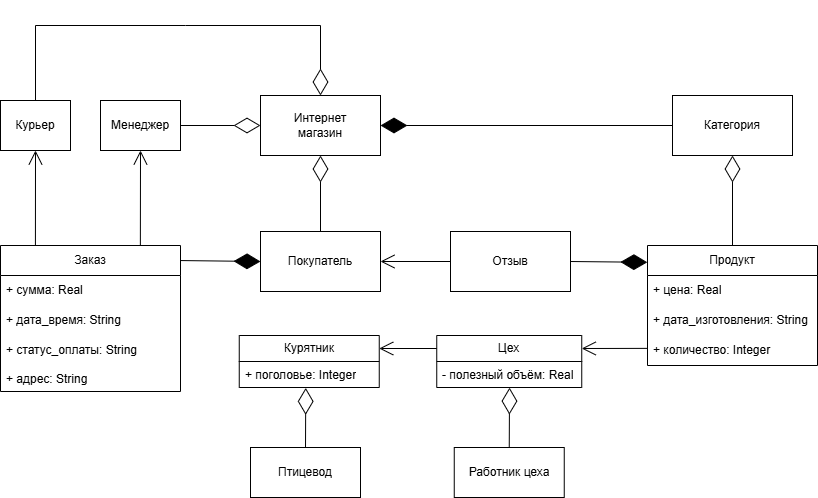
\includegraphics[width=0.9\textwidth]{img/МПО приложение для продажи фермерской продукции.png}
    \caption{МПО приложения для продажи фермерской продукции.}
\end{figure}
\subsubsection{Сущности}
\begin{enumerate}
    \item \textbf{Интернет магазин} - веб-приложение с которым взаимодействует покупатель;
    \item \textbf{Покупатель} - человек желающий приобрести фермерскую продукцию;
    \item \textbf{Отзыв} - мнение покупателя о приобретённом продукте;
    \item \textbf{Продукт} - товар фермерского типа, продаваемый в интернет магазине;
    \item \textbf{Категория} - группа продуктов объединённых по какому-либо признаку;
    \item \textbf{Заказ} - список товаров, которые покупатель желает приобрести;
    \item \textbf{Менеджер} - работник формирующий заказ покупателя;
    \item \textbf{Курьер} - работник доставляющий заказ покупателям;
    \item \textbf{Цех} - здание в котором происходит основная часть процесса производства продукта;
    \item \textbf{Работник цеха} - работник производящий продукт для продажи;
    \item \textbf{Курятник} - здание в котором происходит выращивание кур;
    \item \textbf{Птицевод} - работник ухаживающий за курами.
\end{enumerate}

\newpage

\subsection{Диаграмма коммуникаций}
\subsubsection{Схема}
\begin{figure}[H]
    \centering
    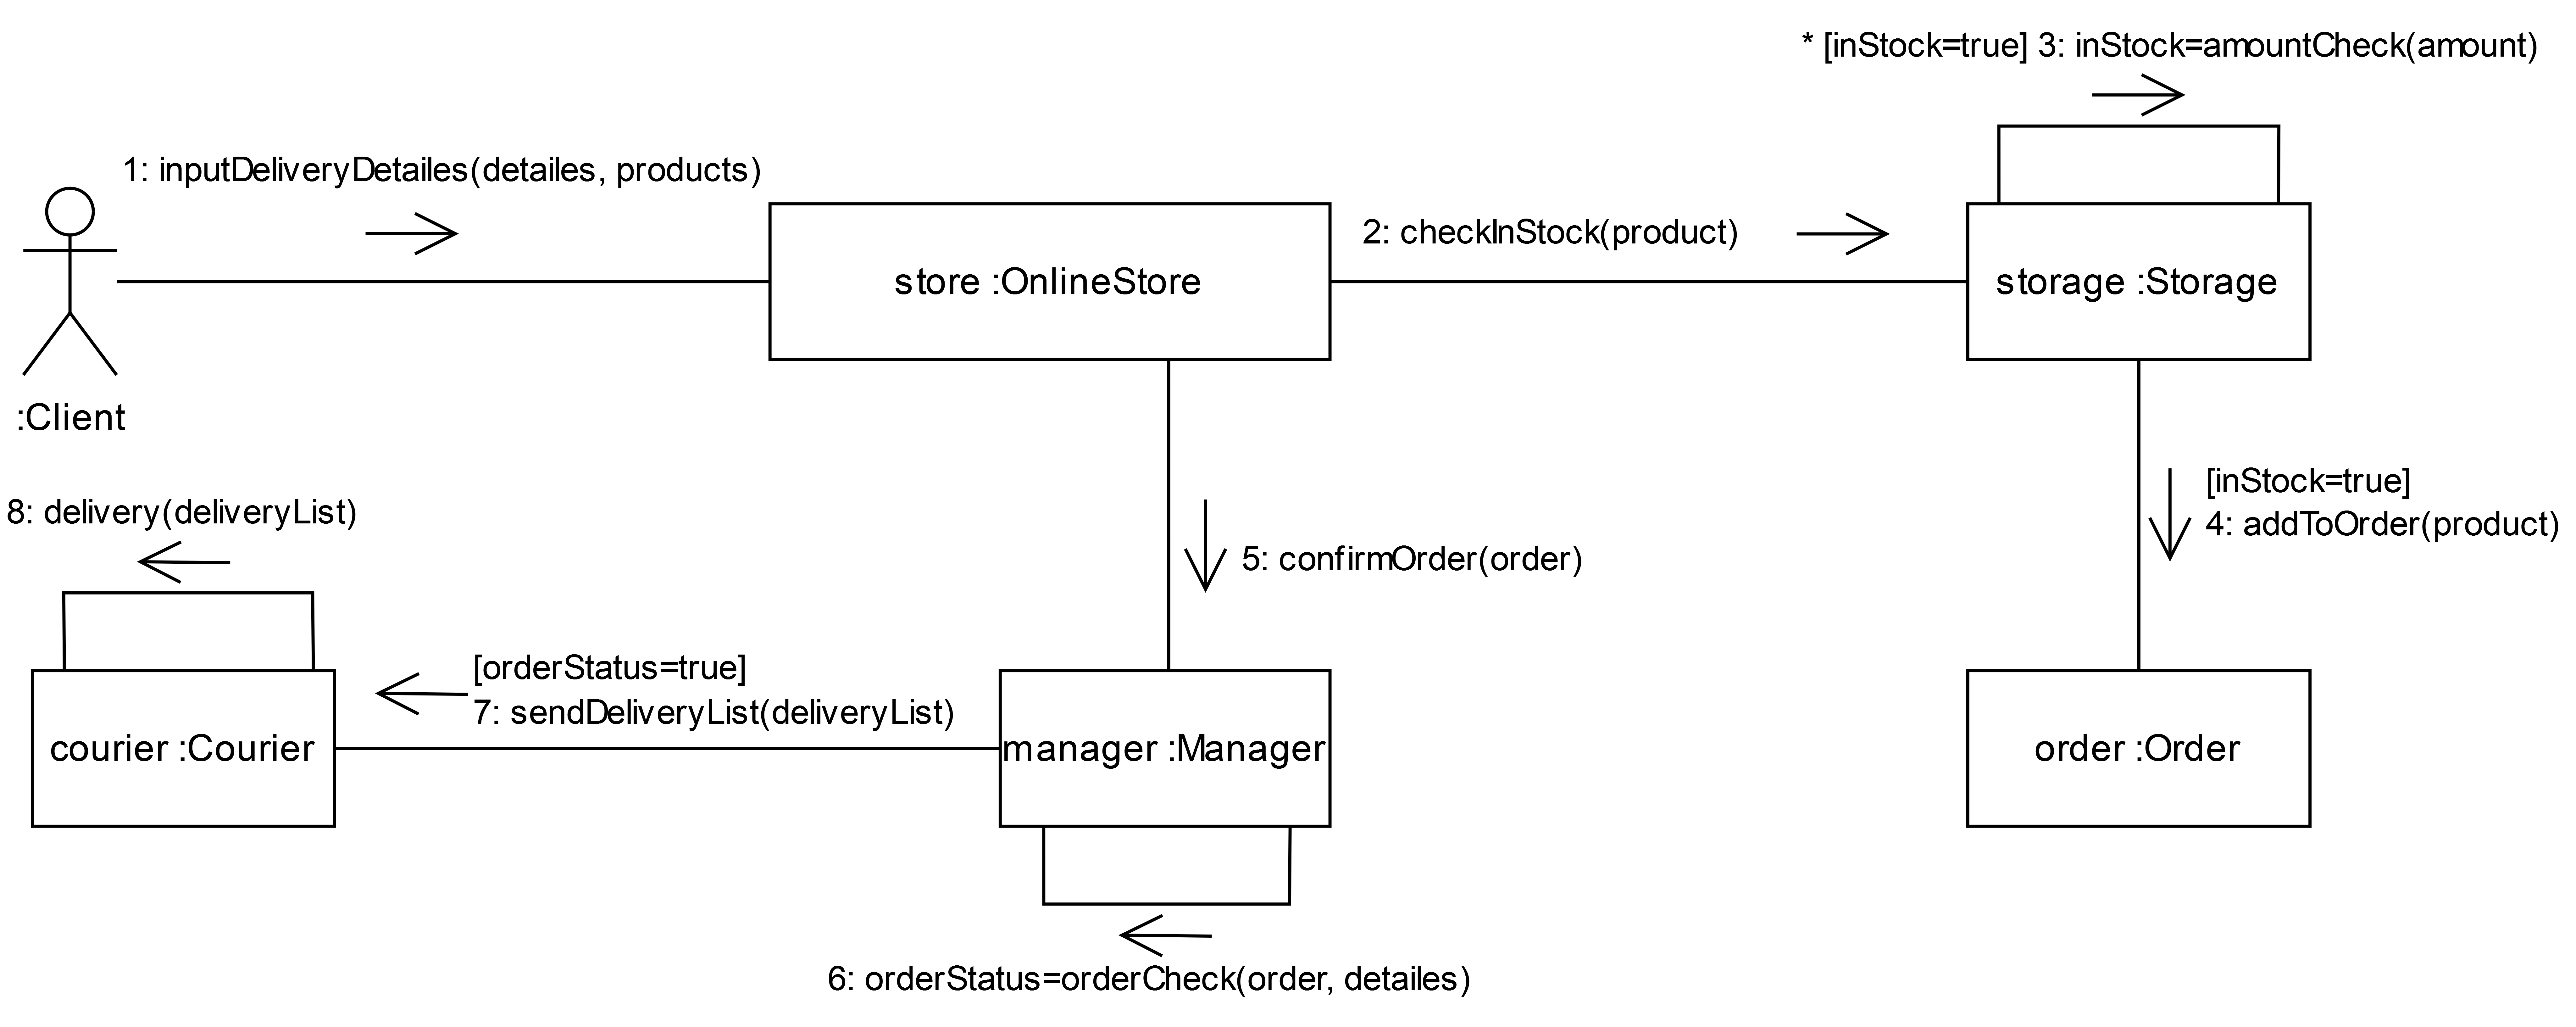
\includegraphics[width=0.9\textwidth]{img/Диаграмма коммуникаций.png}
    \caption{Диаграмма коммуникаций приложения для продажи фермерской продукции.}
\end{figure}
\subsubsection{Описание}
\begin{enumerate}
    \item Пользователь вводит информацию для доставки и выбирает продукты;
    \item[2-3.] Происходит проверка на наличие выбранных продуктов;
    \item[4.] Если продукт есть на складе то он добавляется в заказ;
    \item[5.] Заказ отправляется для проверки менеджеру;
    \item[6.] Менеджер проверяет и уточняет детали заказа;
    \item[7.] Если заказ действительный он передаёт его курьеру;
    \item[8.] Курьер доставляет заказ.
\end{enumerate}

\newpage

\subsection{Диаграмма анализа}
\subsubsection{Схема}
\begin{figure}[H]
    \centering
    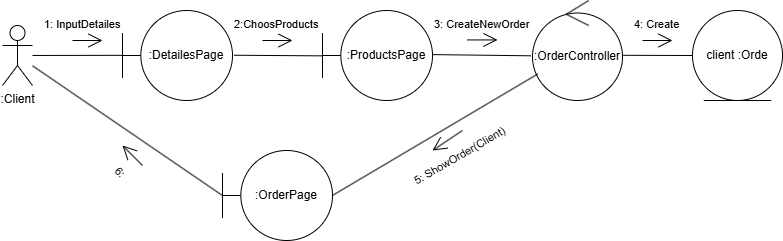
\includegraphics[width=0.9\textwidth]{img/Диаграмма анализа.png}
    \caption{Диаграмма анализа приложения для продажи фермерской продукции.}
\end{figure}
\subsubsection{Описание}
\begin{enumerate}
    \item[1-2.] Пользователь вводит информацию для доставки и выбирает продукты на странице с деталями заказа DetailesPage;
    \item[3.] Пользователь выбирает продукты на станице магазина ProductsPage;
    \item[4.] Граничный класс DetailesPage посылает сообщение контроллеру InStockChecker о том, что необходимо проверить наличие продукта;
    \item[5.] Управляющий объект OrderController создаёт заказ Order;
    \item[6.] Управляющий объект OrderController отображает заказ пользователя на странице заказов OrderPage;
    \item[7.] Пользователь видит станицу заказов OrderPage.
\end{enumerate}
\end{document}